\chapter{Additional measurements on the D\lowercase{y}-K Feshbach spectrum}
\label{Cpt:AddDyKRes}

This chapter is dedicated to the study of Feshbach resonances outside the low-field region that has been the primary focus of our recent efforts. This work has been done in parallel with the studies reported in Chapter \ref{Chpt:Lowfieldpaper} and \ref{Chpt:MolTrap}, and thus with the crucial contributions of Zhu-Xiong Ye and Elisa Soave. In Section \ref{Sec:Compendium}, we explore the interaction spectrum over a large range of magnetic fields and, in Section \ref{Sec:RF217}, we present an attempt to characterize the broad resonance at \SI{217}{G}.



\section{Compendium of  D\lowercase{y}-K Feshbach resonance}
\label{Sec:Compendium}

All of the main results presented in this thesis are obtained working around the interspecies Feshbach resonance close to \SI{7}{G}. While this resonance proved to be a very fruitful tool for studying interspecies interactions and Feshbach molecules, we also invested some time to re-explore the interaction spectrum in the mixture at different magnetic fields, with the objective, and hope, to find other and possibly broader candidates. A similar study was already performed by  previous member of the team, when looking for a strong and broad resonance, which resulted in the identification of the resonance at \SI{217}{G} reported in Ref.~\cite{Ravensbergen2020rif}. However in the years following that study, considerable effort was made to improve the control and stability of the magnetic field in the experiment\footnote{see also Appendix \ref{app:MagneticField} for a presentation of some of the improvements}, which motivated us to re-explore the entire magnetic field range accessible with our experimental setup.

The approach we employed to identify interspecies resonances is the same as the one presented in Sec.~\ref{sec:InterThemScan}. After evaporative cooling of the mixture, always performed at low magnetic fields, we parametrically heat the potassium atomic cloud and then ramp the magnetic field to a target value, at which the two clouds are allowed to thermalize for a fixed amount of time. Strong interspecies interaction corresponds to peaks in the thermalization rate, which we associate with a Feshbach resonance. The magnetic field resolution is of \SI{20}{mG} for fields below \SI{70}{G}, and of \SI{200}{mG} above that. This choice reflects the fact that below \SI{70}{G}, we were looking for \textit{any} resonance, while above that we were focusing only on identifying \textit{broad} resonances, which would justify the additional troubles of working at high magnetic fields. The coarse scan at higher magnetic fields probably missed different narrower features.

The results of this Feshbach spectroscopy are reported in Figures \ref{fig:3_19G_Scan} through \ref{fig:260_360G_Scan}. We identified 35 interspecies Feshbach resonances investigating magnetic fields up to \SI{360}G, which is close to the upper limit of our coils. Ultimately, no suitable broader resonance was found. No other feature broader than the one at \SI{217}{G} was observed, except for a possible candidate around \SI{340}{G} which appeared to have a comparable strength. However, we did not characterize this resonance as we deemed it to be at too high magnetic field, and  both the large number of resonances that would need to be crossed to reach it and the high magnetic field would not allow us to prepare and control efficiently the quantum mixture. All of the others resonances observed are of the order, or narrower, of the \SI{7}{G} resonance, but without the advantage of being at low magnetic field. Table \ref{tab:AllFeshbach} summarize our findings.



\begin{figure}[thb]
	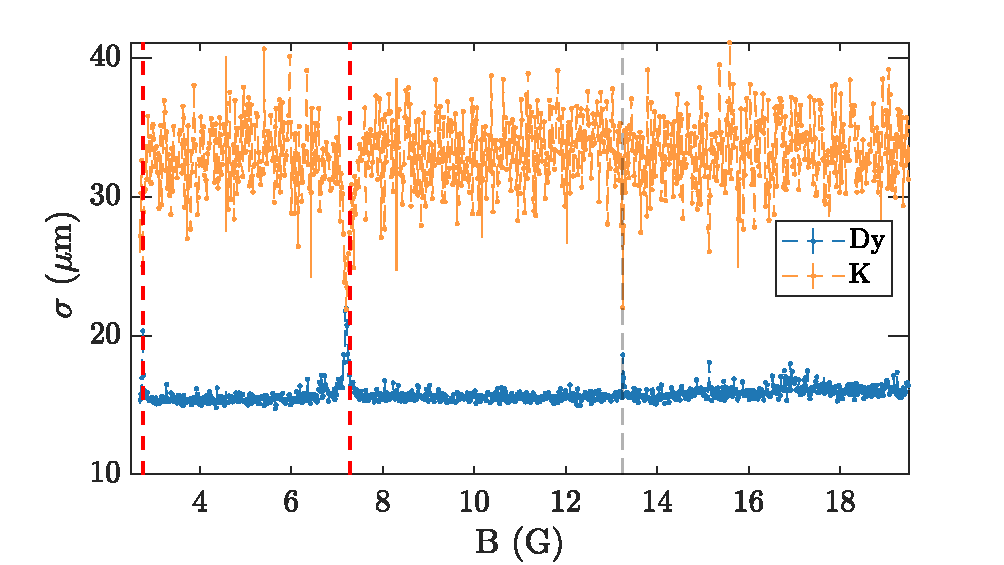
\includegraphics[trim=0cm 0 0cm 0, clip, width=1\columnwidth]{gfx/Cpt6_fig/3_19G.pdf}
	\caption{. \label{fig:3_19G_Scan}}
\end{figure}


\begin{figure}[thb]
	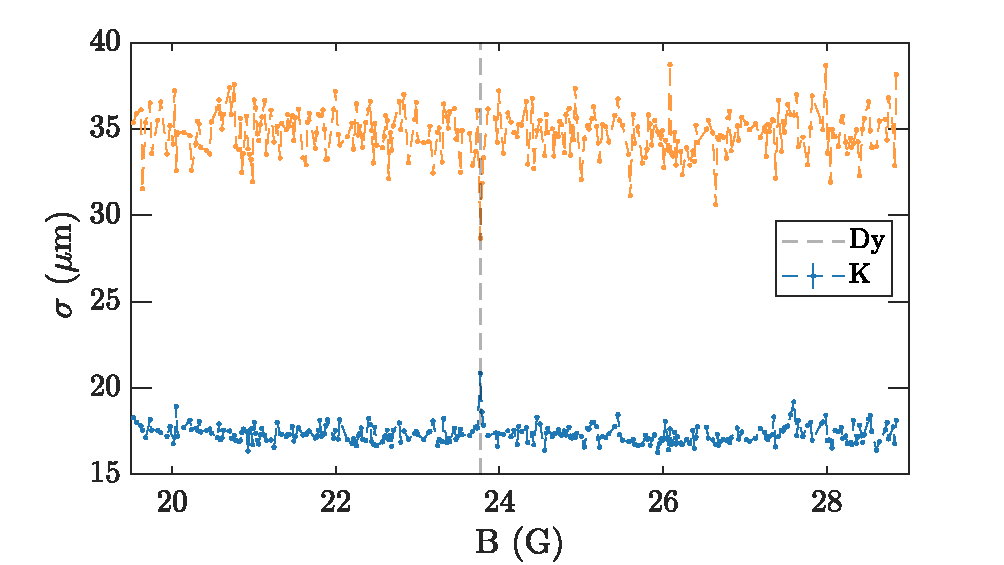
\includegraphics[trim=0cm 0 0cm 0, clip, width=1\columnwidth]{gfx/Cpt6_fig/19_29G.pdf}
	\caption{. \label{fig:19_29G_Scan}}
\end{figure}


\begin{figure}[thb]
	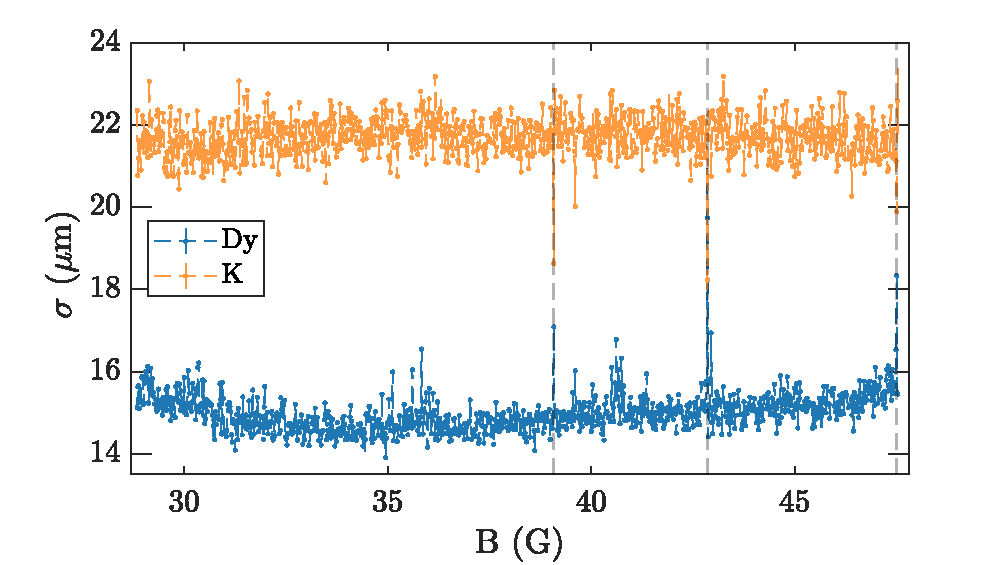
\includegraphics[trim=0cm 0 0cm 0, clip, width=1\columnwidth]{gfx/Cpt6_fig/29_47G.pdf}
	\caption{. \label{fig:29_47G_Scan}}
\end{figure}

\begin{figure}[thb]
	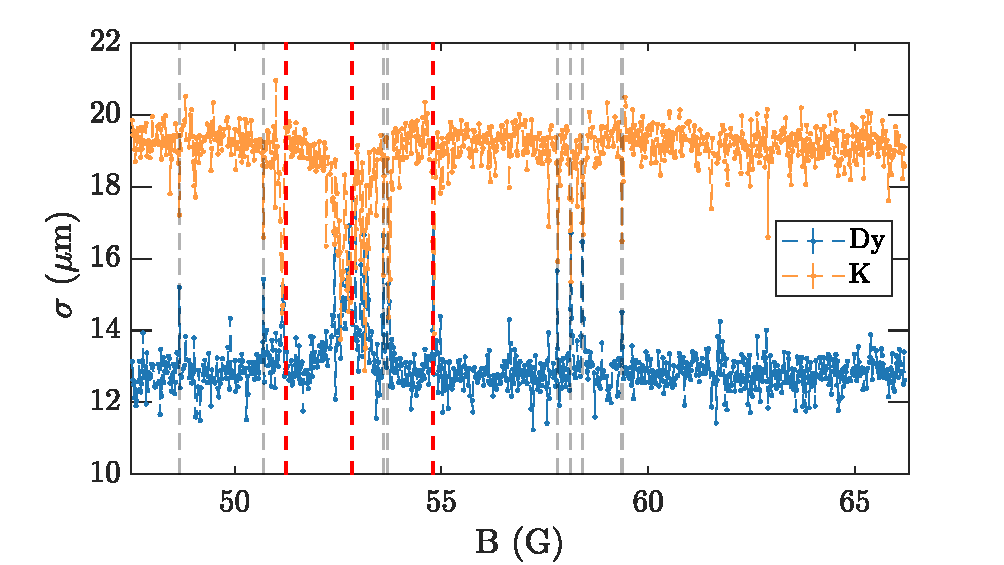
\includegraphics[trim=0cm 0 0cm 0, clip, width=1\columnwidth]{gfx/Cpt6_fig/47_66G.pdf}
	\caption{. \label{fig:47_66G_Scan}}
\end{figure}

\begin{figure}[thb]
	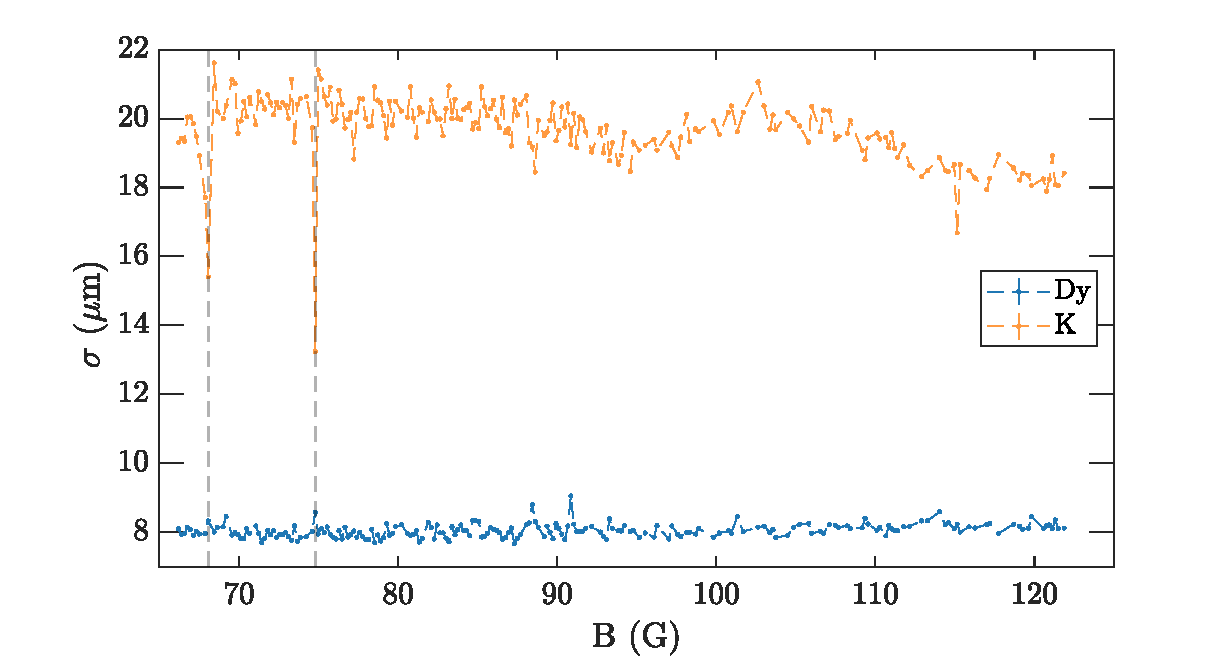
\includegraphics[trim=0cm 0 0cm 0, clip, width=1\columnwidth]{gfx/Cpt6_fig/70_120G.pdf}
	\caption{. \label{fig:70_120G_Scan}}
\end{figure}

\begin{figure}[thb]
	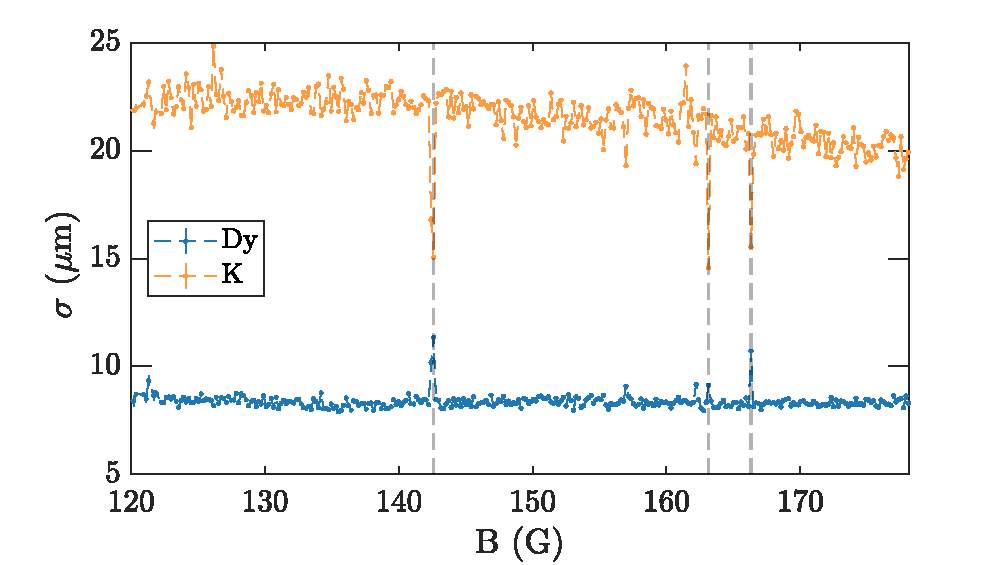
\includegraphics[trim=0cm 0 0cm 0, clip, width=1\columnwidth]{gfx/Cpt6_fig/120_180G.pdf}
	\caption{. \label{fig:120_180G_Scan}}
\end{figure}


\begin{figure}[thb]
	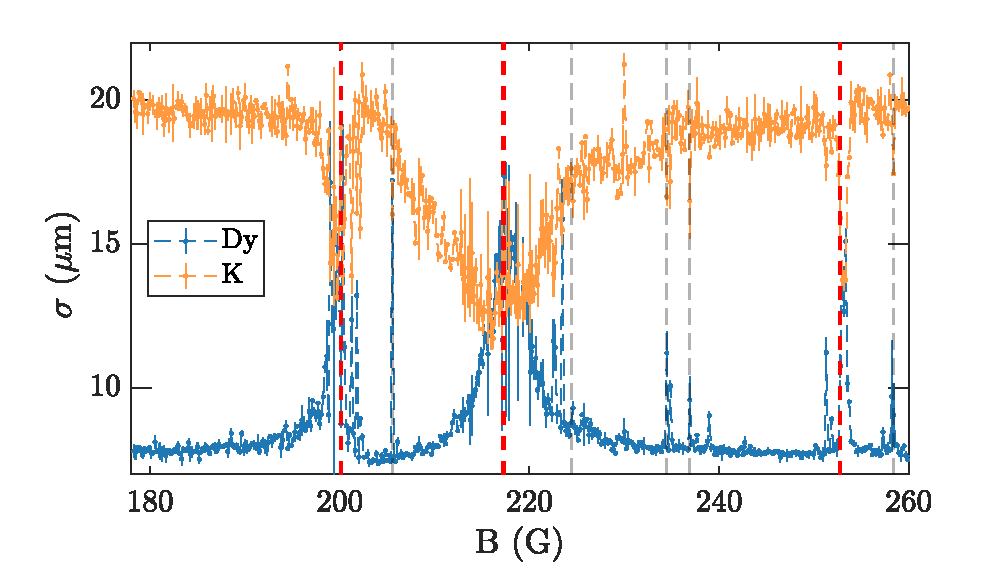
\includegraphics[trim=0cm 0 0cm 0, clip, width=1\columnwidth]{gfx/Cpt6_fig/180_260G.pdf}
	\caption{. \label{fig:180_260G_Scan}}
\end{figure}


\begin{figure}[thb]
	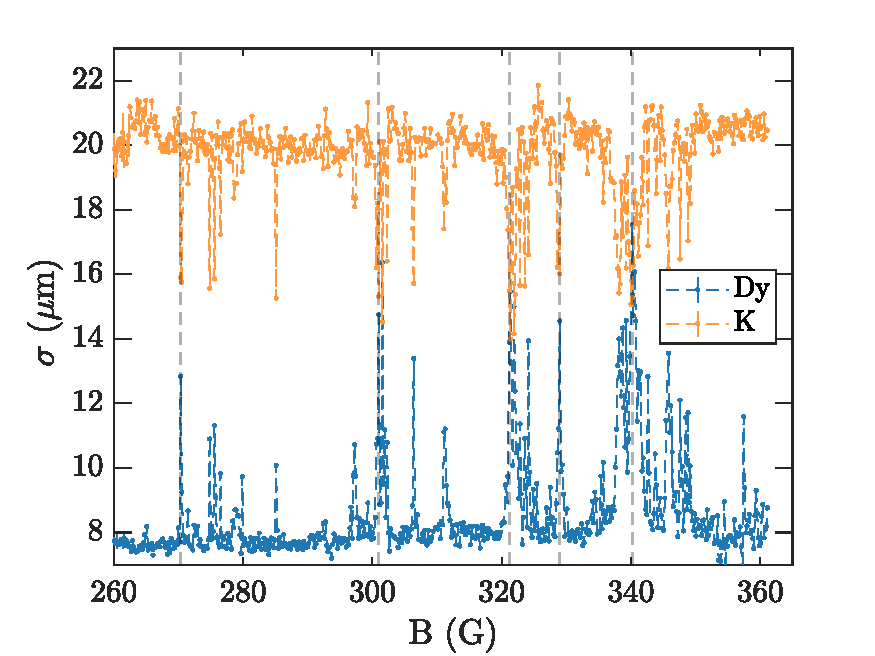
\includegraphics[trim=0cm 0 0cm 0, clip, width=1\columnwidth]{gfx/Cpt6_fig/260_360G.pdf}
	\caption{. \label{fig:260_360G_Scan}}
\end{figure}


\begin{table}[]
	\caption{.}
	
	\medskip
	\begin{center}
		\begin{tabular}{ccc}
			\hline
			\hline
			Magnetic Field (G) \qquad &Resolution\qquad&  Ref. (if available)   \\
			\hline
			$1051.03$     & 0.62 &   \\
			$1064.04$ &  0.50& \\
			$1547.12$& 0.58  &\\
			$2002.00$ & 0.58 &\\
			\hline
			\hline
		\end{tabular}
	\end{center}
	
	\label{tab:AllFeshbach}
\end{table}

\section{RF-spectra of the 217\,G Resonance}
\label{Sec:RF217}



\begin{figure}[thb]
	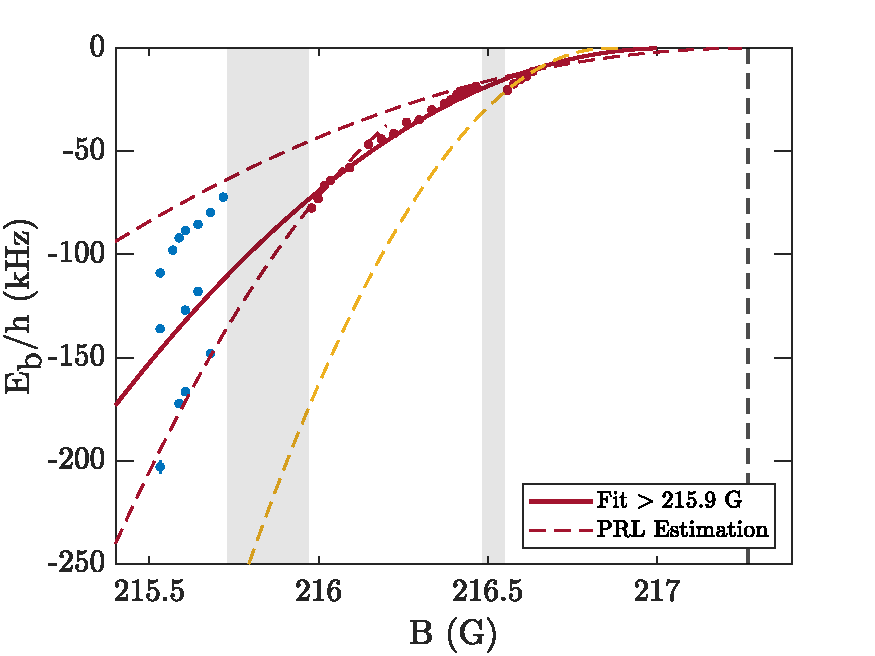
\includegraphics[trim=0cm 0 0cm 0, clip, width=1\columnwidth]{gfx/Cpt6_fig/Binding_energy_217G.pdf}
	\caption{. \label{fig:RF_spectra_217G}}
\end{figure}
